\documentclass[a4paper,10pt]{article}

%%%%%%%%%%%%%%%%%%%%%%%%%%%%%% Packages %%%%%%%%%%%%%%%%%%%%%%%%%%%%%%
\usepackage[a4paper, total={6in, 8in}]{geometry}
\usepackage{parskip}
\usepackage{titlesec}
\usepackage{imakeidx}
\usepackage{hyperref}
\usepackage{layout}
\usepackage{graphicx}

%%%%%%%%%%%%%%%%%%%%%%%%%%%%%% Custom Stuff %%%%%%%%%%%%%%%%%%%%%%%%%%%%%%
%%%%%%%%%%%%%%% Page layout %%%%%%%%%%%%%%%

\setlength{\voffset}{-1in}
\setlength{\textheight}{700pt}

%%%%%%%%%%%%%%%%%%%%%%%%%%%%%% Custom Commands %%%%%%%%%%%%%%%%%%%%%%%%%%%%%%

\newcounter{req}[subsection]
\newcounter{SR}[req]
\newcounter{SSR}[SR]

\renewcommand{\thereq}{\arabic{req}}
\renewcommand{\theSR}{\thereq.\arabic{SR}}
\renewcommand{\theSSR}{\theSR.\arabic{SSR}}

\newcommand{\req}[1]{\refstepcounter{req} \textbf{#1\thereq}}
\newcommand{\SR}[1]{\refstepcounter{SR} \hspace{1.5em} \textbf{#1\theSR}}
\newcommand{\SSR}[1]{\refstepcounter{SSR} \hspace{3em} \textbf{#1\theSSR}}

%%%%%%%%%%%%%%%%%%%%%%%%%%%%%% DOC details %%%%%%%%%%%%%%%%%%%%%%%%%%%%%%
\title{COS720 Project}
\author{u21456552 - Ivan Horak}
\makeindex[intoc]

\begin{document}
\maketitle
\tableofcontents

\pagebreak
%%%%%%%%%%%%%%%%%%%%%%%%%%%%%% Research Overview %%%%%%%%%%%%%%%%%%%%%%%%%%%%%%
\section{Research}

\subsection{How is AI used to detect phishing}

There are a variety of different ways that AI is used to detect phishing
attacks. Some of the more prevalent methods are the use of Machine Learning
models which are trained on large datasets to detect and identify patterns in
phishing attacks, Natural Language Processing is used to understand the context
and intent of communications and to detect manipulation strategies often used
by attackers like urgency. AI is also used not only to identify is some form of
communication is a phishing attack but also to identify comprised accounts and
victims of attacks by monitoring user behaviour for anomalies. Another way that
it is used is to identify phishing attacks that are done by imitating legitimate
websites and people, Computer Vision is often used for this to identify
anomalies in logos or differences compared to legitimate companies and people.
These different strategies for using AI to fight phishing are implemented in
many different ways, they could be implemented on the server side to detect user
anomalies, or they could be a hosted AI with an API endpoint that a plugin could
send data to to get it classified and lastly it could be a feature built into
a tool or application like an email client.\cite{cybersecuritynews} \par

These have a lot of advantages compared to traditional detection methods as
traditional methods rely on humans to define the qualifiers for what is a
phishing attack and then also implement it, however with AI it can adapt and
learn new strategies and even identify unseen phishing tactics that would
usually take a long time to develop using traditional methods.

\subsection{Phishing Detection using AI}

Phishing detection using AI can be defined as the use of any AI strategy to
detect and warn a user or stakeholder about any phishing attacks, especially in
email based phishing attacks, which are one of the most common, AI detection
would be the method that a tool uses to analyze an email and make a prediction
about an email on if it is legitimate or not. AI's role in this is to warn users
of phishing attempts before it is too late, especially users that would
otherwise not know better.


\pagebreak
%%%%%%%%%%%%%%%%%%%%%%%%%%%%%% What is Phishing %%%%%%%%%%%%%%%%%%%%%%%%%%%%%%
\section{What is Phishing and How I Detect it}

To best understand how to implement an AI detection system you need to
understand what is a phishing attack, what are the strategies used in phishing
attacks and what to look out for. \par

Below are the attributes of a phishing email and the signs I look out for:

\begin{itemize}
	\item Does the email contain in links.
	\item Is the email trying to get me to do something
	\item Does the domain of the email address match the claimed domain. (i.e does
	      the email address belong to the same domain as the receiving email address)
	\item Does the name the email set match the name in the email address
	\item Does the email contain phrases like, change password or banking details
\end{itemize}

Given these qualities of a phishing email they are the qualities that I trained
my model on. \par

To do these things I have the following data points:

%%%%%%%%%%%%%%%%%%%%%%%%%%%%%% Model Selection Process %%%%%%%%%%%%%%%%%%%%%%%%%%%%%%
\section{Model Selection Process}

While there are lots of different AI models and techniques that are used to
detecting phishing there are a couple that show up the most in discussions and
implementations. The three that are most prevalent are: Naive Bayes, Logistic
Regression and Random Forest. These are the three that I considered for my
model. \par

I considered Naive Bayes because it works on the probability of a set of
features to be in the same class together and assumes that the features are
independent of each other, which is good for phishing detection since there are
so many different strategies that are used for attacks and different
combinations of strategies. So for my model it needed to be able to consider
data such that it picks up the most common features and the features being able
to come from different emails in the training dataset. \par

Since an email is either a phishing email or not, that binary relationship made
me consider logistic regression as it takes in multiple independent variables
and then a dependent binary variable used for categorization. The binary
dependent variable being if it is phishing or not. \par

Finally I considered Random Forest because of how it can rank features on how
important they were in making a prediction, this is useful as it will naturally
find the features in an email that are most likely to used in a phishing attack
which is needed for phishing detection as sometimes it is only one or two things
in an email that can give away if it is phishing or not and the nature of the
random forest being able to take advantage of this is important. \par

For my implementation I had a couple key requirements, First that it is able to
take in multiple data points, the second that it not be too much overhead to
implement and lastly that there is plenty of documentation on implementation.
This caused me to land on using python for training my model. This is important
for my model selection as it enabled me to rapidly iterate and modify my code to
evaluate different models performances. \par

Due to pythons ease of use and specifically the scikit-learn package I was able
to implement a program that would train all three models at the same time, then
it would feed all three the same data that didn't appear in the datasets used
for training. With this I could easily compare the different models perfomances
and how often each model correctly predicted if the email was legitimate or
not.\par

With this in mind I could then iterate on the training methods and see how the
different models compared and why they made different predictions. And using a
cli implementation I got the models to output the reasoning side by side for
easy comparison. As seen below. \par


\begin{figure}[ht!]
	\centering
	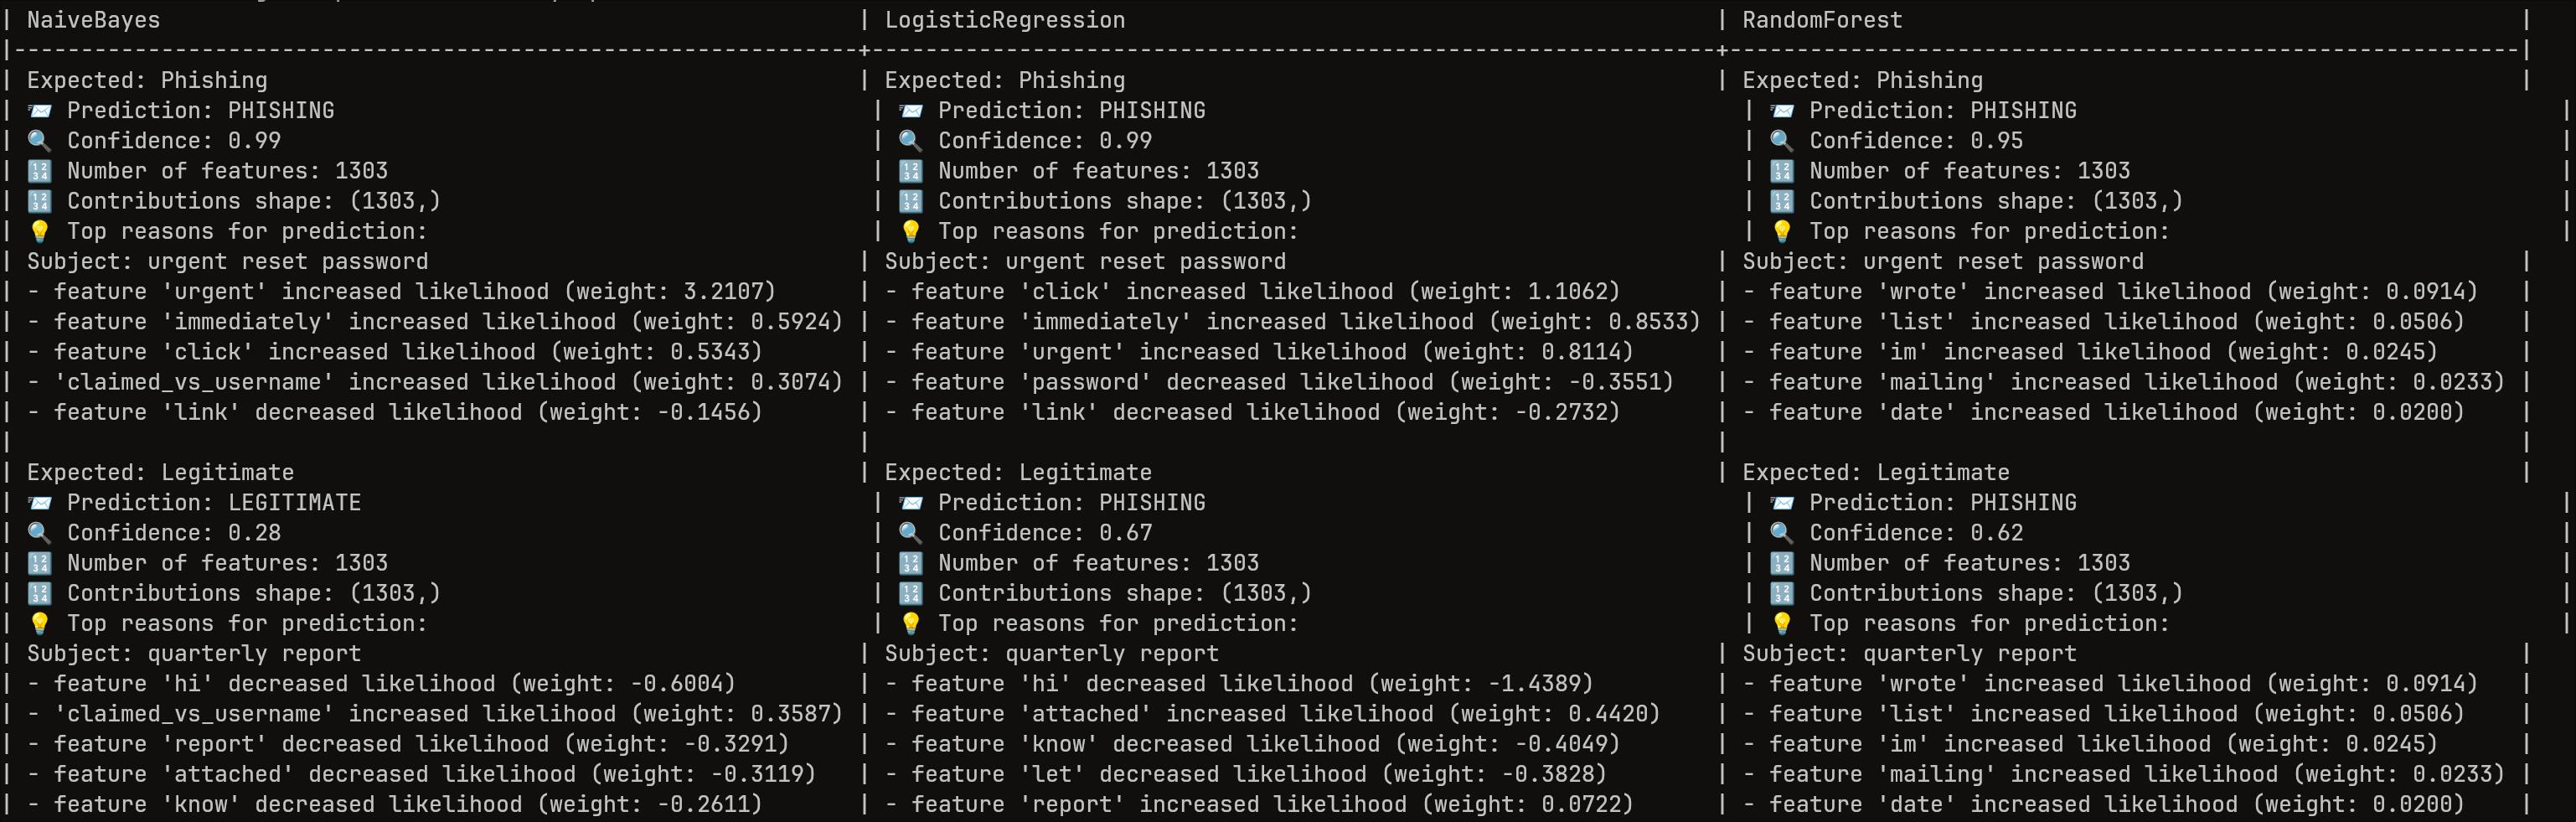
\includegraphics[width=1\textwidth]{doc-img/human_readable_output.jpg}
	\caption{CLI comparison}
	\label{fig:human_readable_output}
\end{figure}

With this information and a simple switch I implemented to toggle it to machine
readable output, I could also get a comparison of how many each model got
correct. As seen below. \par


\begin{figure}[ht!]
	\centering
	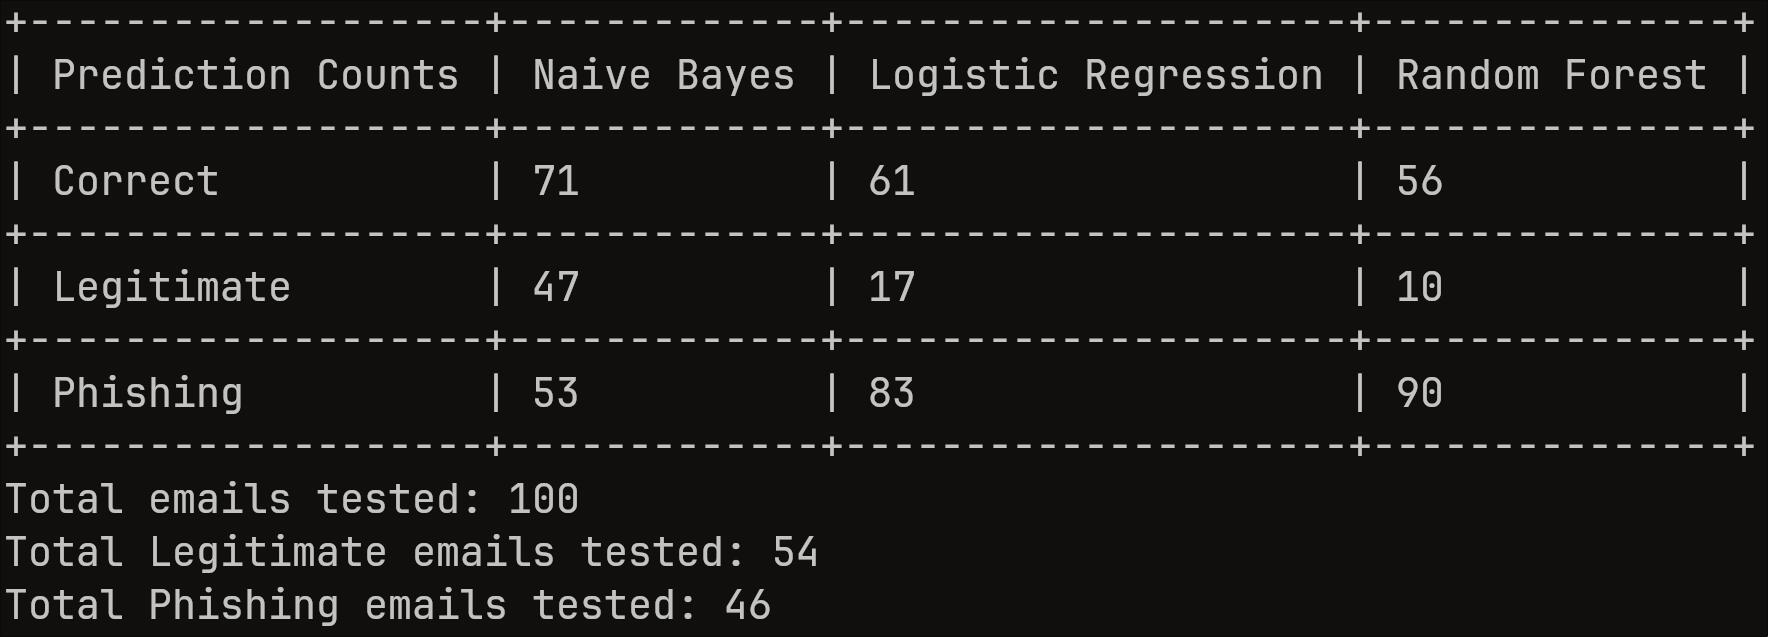
\includegraphics[width=1\textwidth]{doc-img/model-comparison-cli.jpg}
	\caption{Model Comparison}
	\label{fig:model-comparison-cli}
\end{figure}

This led me to choose the Naive Bayes Model as it correctly identifier the most
amount of emails. It also did not drastically prefer either predicting an email
to be phishing or legitimate.

%%%%%%%%%%%%%%%%%%%%%%%%%%%%%% Design %%%%%%%%%%%%%%%%%%%%%%%%%%%%%%
\section{Design}

\subsection{Function Requirements}

\req{R} Model Training

\SR{R} Dataset Preprocessing

\SSR{R} Url detection

\SSR{R} Domain Extraction

\SSR{R} Sender vs Receiver Domain comparison

\SSR{R} Sender email username vs sender claimed identity

\SR{R} Text Cleaning

\SSR{R} Remove HTML from email

\SSR{R} Remove URLS

\SSR{R} Remove stop words

\SSR{R} Remove punctuation

\SR{R} Model Attributes

\SSR{R} Subject, body, sender, receiver attributes

\SSR{R} Url presence

\SSR{R} Are the sender and receiver domains the same

\SSR{R} Is the sender who they claim to be (from username vs name)

\SR{R} Train Model

\SSR{R} Dump Model

\SSR{R} Train model on fitness using dataset

\req{R} Email Analysis/Prediction

\SR{R} Email ingest

\SSR{R} Extract url presence from email

\SSR{R} Extract sender, receiver and identities from email

\SSR{R} Check domains and claimed identity

\SR{R} Prediction output

\SSR{R} Should output if email is legitimate or phishing

\SSR{R} Should give confidence of prediction

\SSR{R} Give features of email and how they affected prediction

\SR{R} Prediction reasoning

\SSR{R} Should give top 5 reasons for prediction

\SSR{R} Should give weighting of reason

\SSR{R} Should say if it increased or decreased likelihood of phishing

\req{R} Frontend

\SR{R} Email input

\SSR{R} Should have input for raw email text

\SSR{R} Should have input for structured email

\SR{R} Result output

\SSR{R} Should display if email is phishing or not

\SSR{R} Should display confidence

\SSR{R} Should display top reasons

\SSR{R} Should display how it affected prediction

\subsection{Security Requirements}

\req{S} API/AI model security

\SR{S} Sanitize/Validate data ingest

\SSR{S} Limit size of input

\SSR{S} Remove any HTML/scrips

\SSR{S} Validate input, e.g. email body, subject, etc.

\SR{S} Application logging

\SSR{S} Log out activity

\SSR{S} Log out errors and exceptions

\SSR{S} Log out access/endpoint usage

\SR{S} Backend Monitoring

\SSR{S} Use APM for activity traces

\SSR{S} Use log ingester like elastic search

\SSR{S} Get metrics using elastic agent

\req{S} Frontend security

\SR{S} Sanitize inputs

\SSR{S} Limit text input lengths

\SSR{S} Validate inputs, e.g. length, type

\SR{S} Application logs

\SSR{S} Log file for user activity

\SSR{S} Log file for errors

\SSR{S} Logs for metrics

\SR{S} DOM purification

\SSR{S} DOM purifier to prevent XSS

\SSR{S} DOM validation/static DOM

\SR{S} Frontend Monitoring

\SSR{S} Use Real User Monitoring (RUM) APM for user observability on the client side

\SSR{S} Get metrics for frontend server

\SSR{S} Ingest frontend logs into elastic search

\pagebreak
\subsection{Use Case Diagrams}

\subsubsection{Model Training}

\begin{figure}[ht!]
	\centering
	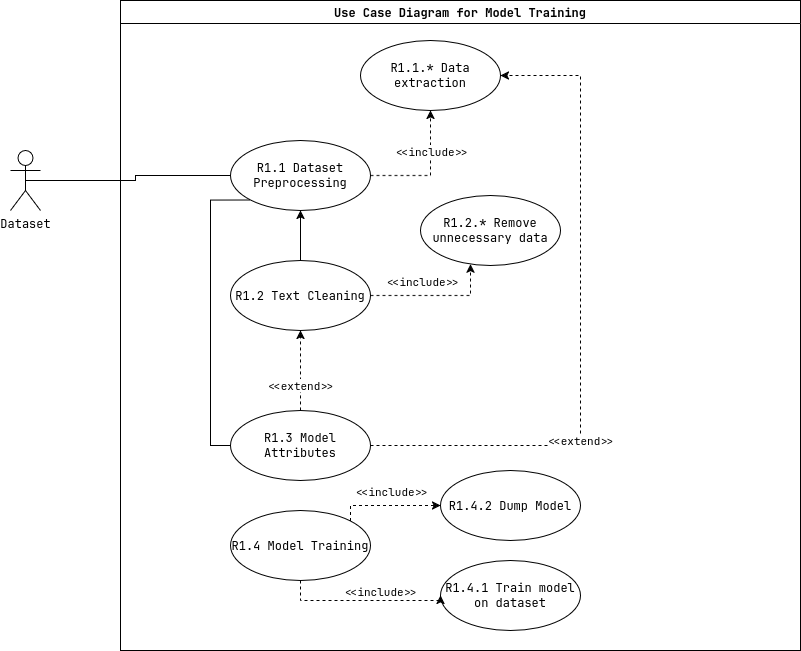
\includegraphics[width=0.8\textwidth]{doc-img/UC-Train-Model.drawio.png}
	\caption{Use Case Diagram on how the model is trained}
	\label{fig:uc-train-model}
\end{figure}

\subsubsection{Model Running/API/Backend}


\begin{figure}[ht!]
	\centering
	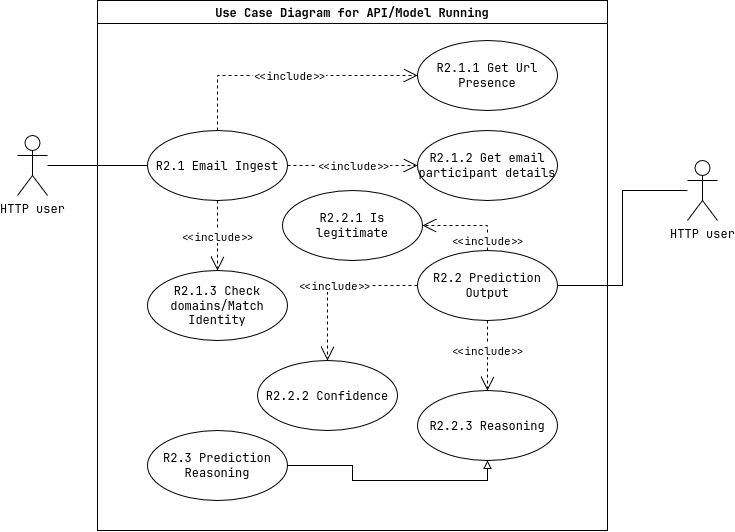
\includegraphics[width=0.8\textwidth]{doc-img/UC-Run-Model.drawio.png}
	\caption{Use Case Diagram for how the Model is run and how the backend works}
	\label{fig:uc-run-model}
\end{figure}

\pagebreak
\subsubsection{Frontend}


\begin{figure}[ht!]
	\centering
	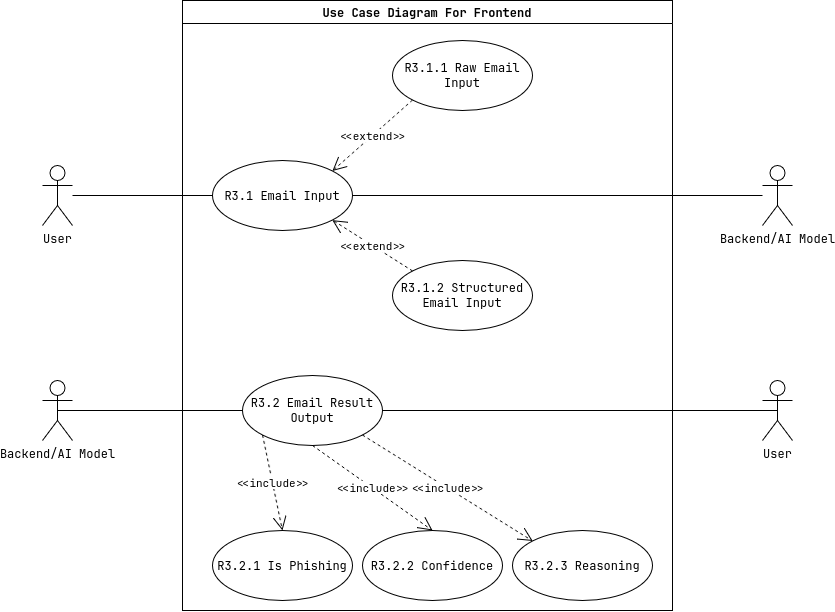
\includegraphics[width=0.8\textwidth]{doc-img/UC-Frontend.drawio.png}
	\caption{Use Case Diagram for how the frontend}
	\label{fig:uc-frontend}
\end{figure}

\subsection{Architectural Diagram}


\begin{figure}[ht!]
	\centering
	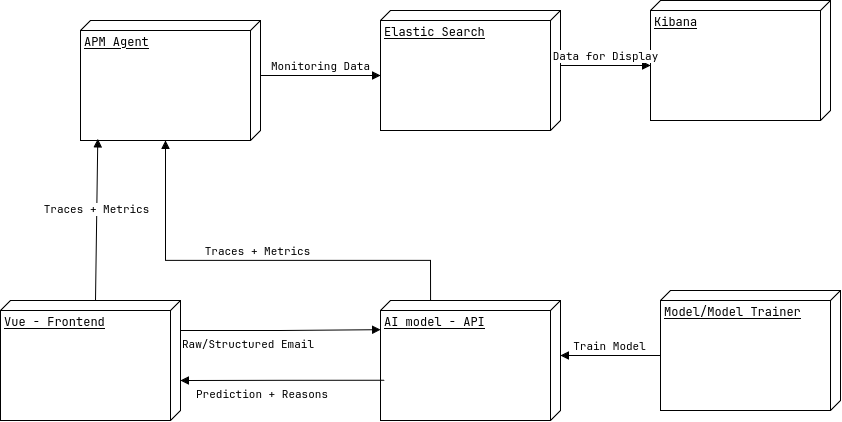
\includegraphics[width=1\textwidth]{doc-img/Arch-Diagram.drawio.png}
	\caption{Architectural Diagram}
	\label{fig:arch-diagram}
\end{figure}

\pagebreak
%%%%%%%%%%%%%%%%%%%%%%%%%%%%%% How it works %%%%%%%%%%%%%%%%%%%%%%%%%%%%%%
\section{How the Model works and what it does}

\subsection{Preprocessing}

In the preprocessing step I ingest the data from multiple datasets from the
phishing dataset provided to use. In this ingestion I first load and normalize
the data in a loop over the different csv's. I load the data into dataframes
from pandas. \par

The first step in my preprocessing is to detect if there is a URL
in the email, first by checking if that was provided by the dataset and if not
the body and subject are scanned to detect the presence of any URLs. \par

The next step is splitting out the senders domain and receivers domain and then
adding a boolean to the dataframe entry which represents whether the sender's
domain is the same as the receiver's domain. This is to train it for phishing
attacks that come from outside an organization. \par

Next the senders claimed name (i.e the part of the sender header before the
email address, e.g. "From: John Doe <john.doe@company.com>") as well as the
username of the email address are extracted, then a similarity is calculated
using the levenshstein distance of the strings which is the number of
single-character edits required to change one word into another. This is usefull
for training the model on phishing detection as many phishing tactics involve
pretending to be someone else. The levenshstein distance is used to account for
the fact that rarely does someones claimed name fully match their username. \par

Finally I clean and remove all stopwords from the subject and body of the email.
This is to ensure that only words and details that impact the meaning and intent
of the email are left over and are used in the training process. This is
important as if the text wasn't cleaned then the most common words will effect
the models predictions in negative ways. \par

\subsection{Model output - confidence/feature highlights}

The main outputs for the model/api are the prediction which is either "phishing"
or "legitimate" these are based on the confidence, if the confidence is higher
than 0.5 then the email is labled as phishing else it is labled as legitimate.
Along with the prediction the confidence is also output so that a user would be
able to evaluate the chances of it being phishing or not. \par

The other thing that is output is the top 5 features that contributed to the
prediction along with if the feature increased or decreased the likelihood of
the email being phishing and finally the weighting by which the feature effected
the prediction.\par

The different kinds of features that could be outputed are the different words
that contributed, if the claimed vs actual identity were the same, the presence
of a url and if the domains matched. \par

\subsection{Model Performance}

In the development of the model I made a csv with 100 entries, made up of a
mixture of legitimate and phishing emails, none of these emails appeared in the
training data. \par

This csv of emails was used to evaluate how well the model performed over
iterations and allowed me to compare the performance and accuracy of different
models, either previous iterations of the model or completely different machine
learning strategies. Using this dataset I managed to get my final model to
correctly identity 71 of the 100 emails. This is a high success rate considering
the complexity of the task. The model also tended to identify emails as phishing
rather than legitimate most of the time. This is preferable as it is better to
tend to the side of caution rather than labeling emails as legitimate when they
aren't. \par

\pagebreak
\subsection{Model Performance Metrics}

\begin{figure}[ht!]
	\centering
	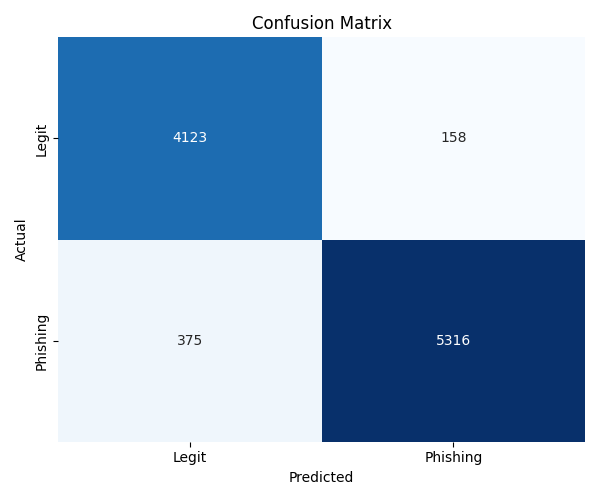
\includegraphics[width=0.8\textwidth]{model_performance/NaiveBayes/confusion_matrix.png}
	\caption{Naive Bayes Confusion Matrix}
	\label{fig:confusion-matrix}
\end{figure}

\begin{figure}[ht!]
	\centering
	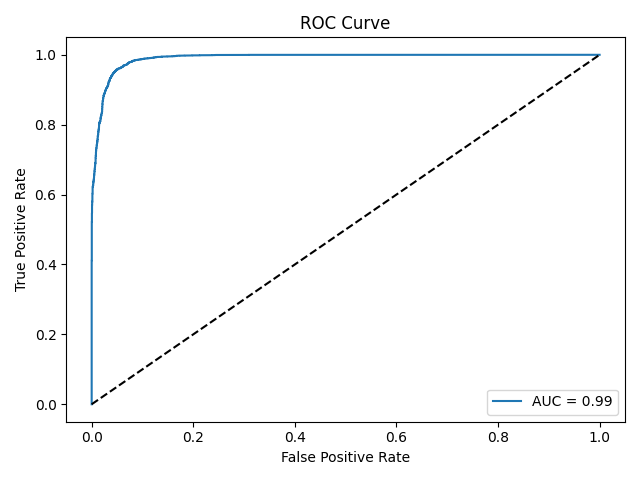
\includegraphics[width=0.8\textwidth]{model_performance/NaiveBayes/roc_curve.png}
	\caption{Naive Bayes ROC Curve}
	\label{fig:roc-curve}
\end{figure}

\begin{figure}[ht!]
	\centering
	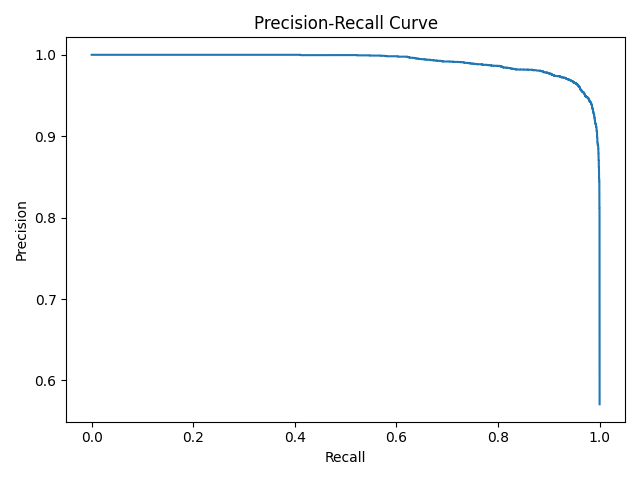
\includegraphics[width=0.8\textwidth]{model_performance/NaiveBayes/precision_recall_curve.png}
	\caption{Naive Bayes Precision Recall Curve}
	\label{fig:precision-recall-curve}
\end{figure}

%%%%%%%%%%%%%%%%%%%%%%%%%%%%%% Security Features %%%%%%%%%%%%%%%%%%%%%%%%%%%%%%
\section{Security Features}

\subsection{Frontend}

To ensure that the frontend of my application is secure I tried to follow and
treat the application as if it would actually be deployed. With this in mind the
following are security features I implemented on the Vue frontend:

\begin{itemize}
	\item I used the dompurify package which is an XSS sanitizer for HTML
	\item I did input validation on the inputs for the raw email input and
	      structured email inputs
	\item I limited input lengths to the lengths found in the RFC documents for
	      emails
\end{itemize}

I also added some observability features to better monitor the application for
possible attacks or vulnerabilities.

\begin{itemize}
	\item I used the RUM APM monitoring from elastic search to get client side
	      metrics and traces.
	\item I also used elastic search to monitor the machine metrics that the
	      application is running on for high resource usage.
	\item I added logging to a file to ensure that if the application goes down or
	      there is unusual activity there is some trace to follow for an
	      investigation.
	\item I also integrated with kibana to view the metrics and service traces as
	      well as any logs that the application produces.
\end{itemize}

\subsection{Backend}

For the backend there is also a variety of security features that I implemented,
including logging and error handling.

The most important security features for the running of the backend are:

\begin{itemize}
	\item Proper error handling and exception handling.
	\item Type checking for inputs.
	\item I also added input sanitization and validation with the same kinds of
	      rules as the inputs for the frontend.
\end{itemize}

I also wanted to ensure proper observability for the backend so to ensure that
any unusual activity is monitored and detected I integrated it using the
FastApi/Starlette Elastic APM agent and I added logging to a file for proper
persistence of any activity. The main features of these are:

\begin{itemize}
	\item Elastic Search database for log ananlysis and storage
	\item Kibana for metrics observability and ananlysis
	\item Loggin to a file including timestamps, requests and other important
	      details.
\end{itemize}

\subsection{ElasticSearch and Kibana}


\begin{figure}[h]
	\centering
	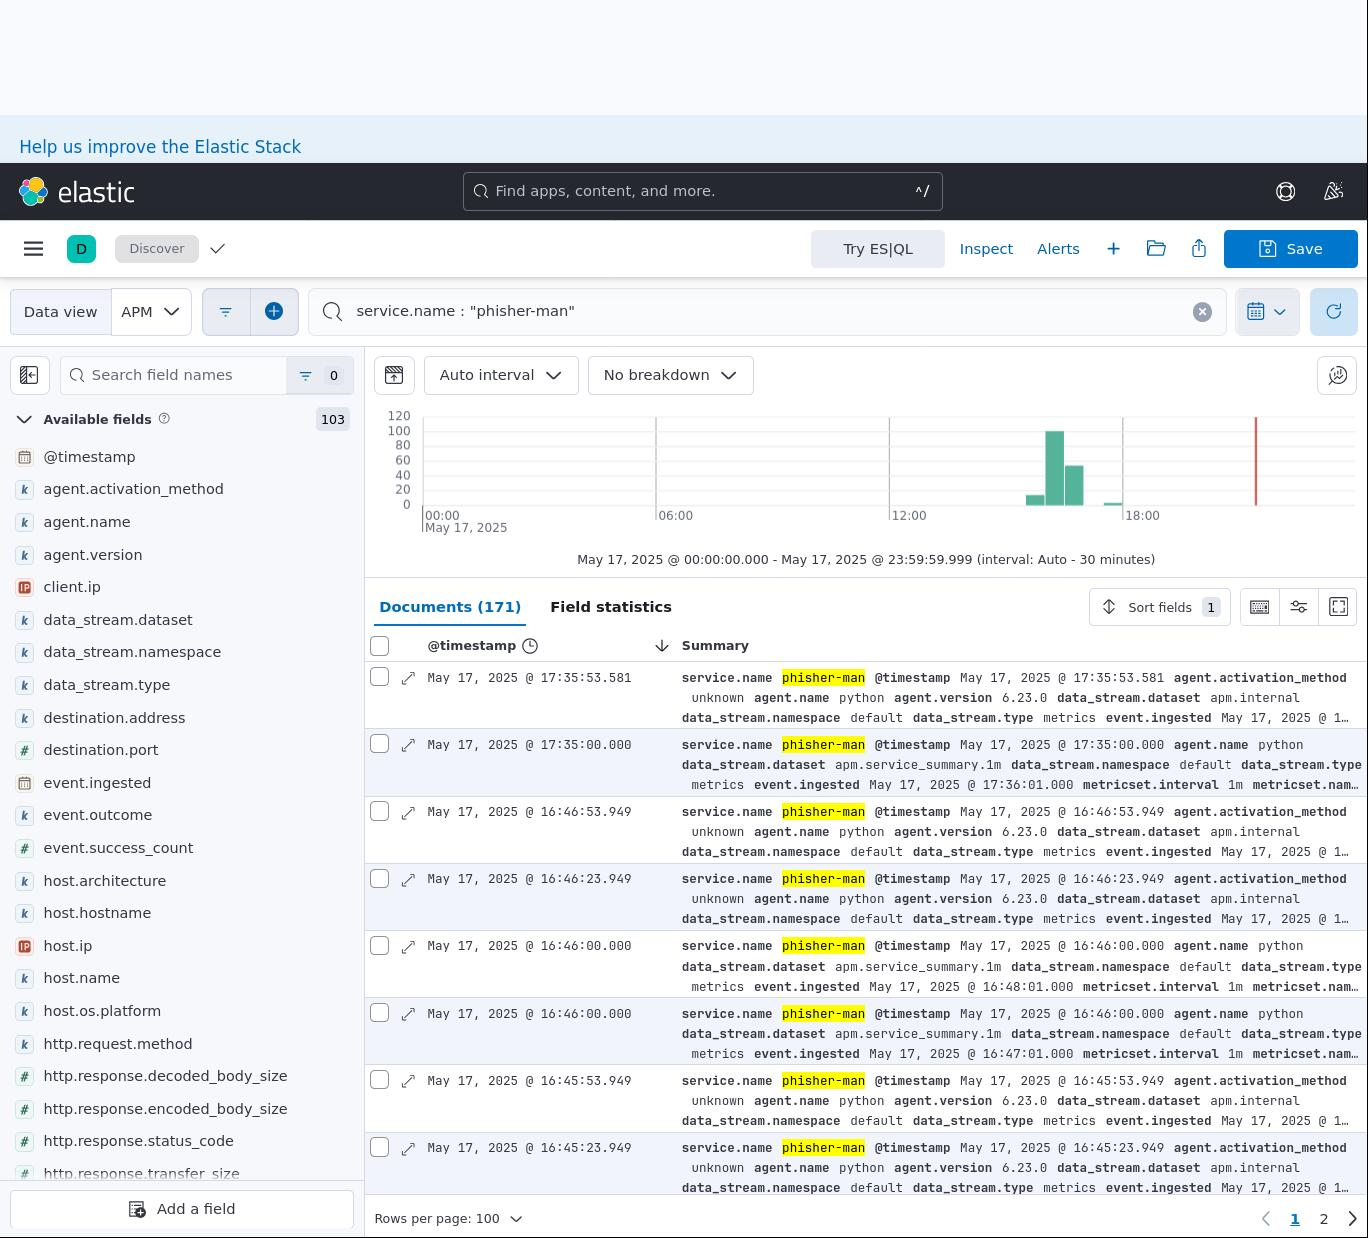
\includegraphics[width=0.8\textwidth]{doc-img/kibana-logs.jpg}
	\caption{Kibana log streams}
	\label{fig:kibana-logs}
\end{figure}

%%%%%%%%%%%%%%%%%%%%%%%%%%%%%% Code Base %%%%%%%%%%%%%%%%%%%%%%%%%%%%%%

\section{Code Base}

\subsection{Dependencies}

\subsection{Docker}

To be able to run this project with the APM monitoring make sure to run the
command 'docker compose up -d' in the home directory of this project.

\subsubsection{Frontend}

The project is split into two areas for proper separation of concerns. The first
area is the frontend which is a Vue project since it is one of the easiest
frontend frameworks to work with and the npm packages mean that implementing and
maintaining features should be easy. Vue is also one of the most modern frameworks
and has a very active community. This means that it is well maintained and most
security concerns have already been addressed or there is a package for it.\par

To install the dependencies for the vue project, ensure that you have nodejs
installed and then cd into the email-parser-ui directory and run 'npm
install'.\par

\subsubsection{Backend}

For the backend I used python as it has a lot of libraries for machine learning
and also it has a very simple recognisable syntax which makes it easy to
understand and code and maintain. I also used FastApi in python to create the
endpoints that are used for the frontend. \par

To install the dependencies I recommend using 'uv' which is a python virtual
environment manager written in rust for speed and easy setup. To install all the
dependencies with uv run the command 'uv sync'. Then to activate the virtual
environment run 'source .venv/bin/activate'. This will make all the packages and
tools for the project available.\par

\subsection{Starting the applications}

\subsubsection{Frontend}

To start the Vue frontend run the command 'npm run dev'.

\subsubsection{Backend}

Now to start the API run 'uvicorn app.main:app --reload' this will start the
API. \par

\subsection{Accessing the UI}

To be able to see the frontend there should be a link in the output from
starting the vue frontend that will serve the vue frontend. The python backend
is always accessible by 'http://localhost:8000/' and the swagger docs are
accessible at 'http://localhost:8000/doc'. \par

The kibana portal is accessible at 'http://localhost:8200'.\par

\subsection{Code Repository}

The code in this project is accessilbe at 'https://github.com/ChuufMaster/phisher-man'. \par

\pagebreak
%%%%%%%%%%%%%%%%%%%%%%%%%%%%%% Bibliography %%%%%%%%%%%%%%%%%%%%%%%%%%%%%%
\section{Bibliography}
\bibliographystyle{ieeetr}
\bibliography{bibliography}

%%%%%%%%%%%%%%%%%%%%%%%%%%%%%% Index %%%%%%%%%%%%%%%%%%%%%%%%%%%%%%
\printindex

\end{document}
